\documentclass[../main-sheet.tex]{subfiles}
\usepackage{../style}
\backgroundsetup{contents={}}
\begin{document}
\chapter{Boolean Algebra}
\section{Boolean Expressions}
\begin{defn}
    Let $ x_1,x_2,\dots,x_n $ be a set of $ n $ variables (or letters or symbols). A \emph{Boolean Polynomial (Boolean expression, Boolean form or Boolean formula)} $ p(x_1,x_2,\dots,x_n) $ in the variables $ x_1,x_2,\dots,x_n $ is defined recursively as follows:
    \begin{enumerate}
        \item The symbols $ 0 $ to $ 1 $ are Boolean polynomials\label{en:1}
        \item $ x_1,x_2,\dots,x_n $ are all Boolean polynomials
        \item if $ p(x_1,x_2,\dots,x_n) $ and $ q(x_1,x_2,\dots,x_n) $ are two Boolean polynomials, then so are
        \[
            p(x_1,x_2,\dots,x_n)\lor q(x_1,x_2,\dots,x_n)
        \]
        and
        \[
            p(x_1,x_2,\dots,x_n)\land q(x_1,x_2,\dots,x_n)
        \]
        \item If $ p(x_1,x_2,\dots,x_n) $ is a Boolean polynomial, then so is $ (p(x_1,x_2,\dots,x_n))' $.\label{en:4}
        \item There are no Boolean polynomials in the variables $ x_1,x_2,\dots,x_n $ other than those obtained in accordance with rules \ref{en:1} to \ref{en:4}.
    \end{enumerate}
\end{defn}
Thus, Boolean expression is an expression built from the variables given using Boolean operations $ \lor $, $ \land $ and $ ' $.


For example, for variable $ x,y,z $, the expression
\begin{align*}
    p_1(x,y,z)&=(x\lor y)\land z\\
    p_2(x,y,z)&=(x\lor y')\land (y\land 1)\\
    p_3(x,y,z)&=(x\lor (y'\land z))\lor (x\land (y\land 1))
\end{align*}
are Boolean expressions.

Notice that a Boolean expression is $ n $ variable may or may not contain all the $ b $ variables. Obviously, an infinite number of Boolean expressions may be constructed in $ n $ variables.
\begin{defn}[Literal]
    A \emph{literal} is a variable or complemented variable such as $ x $, $ x' $, $ y $, $ y' $, and so on.
\end{defn}
\begin{defn}[Fundamental Product]
    A \emph{fundamental product} is a literal or a product of two or more literal in which no two literal involve same variable.
\end{defn}
For example, 
\[
    x\land z',\;x\land y'\land z,\;x,\;y'\;x'\land y\land z
\]
are fundamental products whereas
\[
    x\land y\land x'\land z \text{ and } x\land y\land z\land y
\]
are not fundamental products.
\begin{rem}
    Fundamental product is also called a \emph{minterm} or \emph{complete product}. In what follows we shall denote $ x\land y $ by $ xy $.
\end{rem}
Any product of literals can be reduced to either 0 or a fundamental product.

For example, consider $ x $ $ y $ $ x' $ $ z $. Since, $ x\land x'=0 $ by complement law, we have $ xyx'z=0 $.

Similarly, if we consider $ x\;y\;z\;y $ then since $ y\land y=y $ (idempotent law), we have $ xyzy=xyz $, which is a fundamental product.
\begin{defn}
    A fundamental product $ P_1 $ is said to be contained in (or included in) another fundamental Product $ P_2 $ if the literals of $ P_1 $ are also literals of $ P_2 $.\\
    For example, $ x'z $ is contained in $ x'yz $ but $ x'z $ is not contained in $ xy'z $ since $ x' $ is not a literal of $ xy'z $.
\end{defn}
Observe that if $ P_1 $ is contained in $ P_2 $, say $ P_2=P_1\land Q $, then, by the absorption law,
\[
    P_1\lor P_2=P_1\lor (P_1\land Q)=P_1
\]
For example,
\[
    x'z\lor x'yz=x'z
\]
\begin{defn}
    A Boolean expression $ E $ is called a sum-of-products expression(disjunctive Normal Form or DNF) if $ E $ is a fundamental product or the sum (join) of two or more fundamental products none of which is contained in another.
\end{defn}
\begin{defn}
    Two Boolean expression $ P(x_1,x_2,\dots,x_n)$ and $ Q(x_1,x_2,\dots,x_n)$ are called equivalent (or equal) if one can be obtained from the other by a finite number of applications of the identities of a Boolean algebra.
\end{defn}

\begin{defn}
    Let $ E $ be any Boolean expression. A sum of product form of $ E $  is an equivalent Boolean sum of products expression.\\
    Example: Consider the expression
    \[
        E_1(x,y,z)=xz'+y'z+xyz'
    \]
    Although the expression $ E_1 $ is a sum of products, it is not a sum-of-products expression because, the product $ xz' $ is contained in the product $ xyz' $. But, by absorption law, $ E_1 $ can be expressed as
    \[
        E_1(x,y,z)=xz'+y'z+xyz'=xz'+xyz'+y'z=xz'+y'z
    \], 
    which is a sum-of-product form for $ E_1 $.
\end{defn}
\section{Algorithm for Finding Sum-of-Products Forms}
The input is a Boolean expression $ E $. The output is a sum-of-products expression equivalent to $ E $.
\begin{enumerate}[label=Step \arabic*.]
    \item Use De Morgan's Law and involution to move the complement operation into any parenthesis until finally the complement operation only applies to variables. Then $ E $ will consist only sums and products of literals.
    \item Use the distributive operation to next transform $ E $ into a sum of
    products.
    \item Use the commutative, idempotent, and complement laws to transform each product in $ E $ into 0 or a fundamental product.
    \item Use the absorption law and identity law to finally transform $ E $ into a sum of products expression.
\end{enumerate}
For example, we apply the above Algorithm to the Boolean expression,
\[
    E=((xy)'z)'((x'+z)(y'+z'))'
\]
\begin{enumerate}[label=Step \arabic*.]
    \item Using De Morgan's laws and involution, we obtain
    \begin{align*}
        E&=((xy)''+ z') ((x'+ z) + (y'+z')')\\
        &=(xy+z') (x z' + y z)
    \end{align*}
    Thus $ E $ consists only of sum and products of literals.
    \item Using the distributive laws, we obtain
    \begin{align*}
        E&=(xy+z') (x z' + y z)\\
        &=xyxz'+xyyz+xz'z'+yzz'
    \end{align*}
    Thus $ E $ is now a sum of products.
    \item Using commutative idempotent and complement law, we obtain
    \[E=xyz'+xyz+xz'+0\]
    Each term in $ E $ is a fundamental product or 0.
    \item The product $ xz' $ is contained in $ xyz' $; hence, by the absorption law,
    \[
        xz'+(xz'y)=xz'
    \]
    Thus we may delete $ xyz' $ form the sum. Also, by the identity law for 0, we may delete 0 from the sum. Accordingly,
    \[
        E=xyz+xz'
    \]
    $ E $ is now represented by a sum-of-products expression.
\end{enumerate}
\section{Consensus of Fundamental Products}
Let $ P_1 $ and $ P_2 $ be fundamental products such that exactly one variable say $ x_k $ appears uncomplemented in one of $ P_1 $ and $ P_2 $ and complemented in the other. Then the \emph{consensus of $ P_1 $ and $ P_2 $} is the product (without repetitions) of the literals of $ P_1 $ and $ P_2 $ after $ x_k $ and $ x_k' $ are deleted. (we do not define the consensus of $ P_1=x $ and $ P_2=x' $)
\begin{lem}
    Suppose $ Q $ is the consensus of $ P_1 $ and $ P_2 $. Then $ P_1 + P_2 + Q = P_1 + P_2 $.
\end{lem}
\begin{proof}
    Since the literals commute, we can assume without loss of generality that
    \[
        P_1=a_1a_2\dots a_r t \qquad P_2=b_1b_2\dots b_s t' \qquad Q=a_1a_2\dots a_rb_1b_2\dots b_s
    \]
    Now, $ Q = Q(t+t') = Qt+Qt' $. Because $ Qt $ contains $ P_1 $, $ P_1+Qt = P_1 $; and because $ Qt' $ contains $ P_2 $, $ P_2+Qt' = P_2 $.
    Hence,
    \begin{align*}
        P_1+P_2+Q&=P_1+P_2+Qt+Qt'\\
        &=(P_1+Qt)+(P_2+Qt')\\
        &=P_1+P_2.
    \end{align*}
\end{proof}
\begin{prob}
    Find the consensus $ Q $ of $ P_1 $ and $ P_2 $, where
    \begin{enumerate}[label=(\roman*)]
        \item $ P_1=xyz's $, $ P_2=xy't $
        \item $ P_1=xy' $, $ P_2=y $
        \item $ P_1=x'yz $, $ P_2=x'yt $
        \item $ P_1=x'yz $, $ P_2=xyz' $.
    \end{enumerate}
\end{prob}
\begin{soln}
    \hfill
    \begin{enumerate}[label=(\roman*)]
        \item $ P_1=xyz's $, $ P_2=xy't $\\
        Delete $ y $ and $ y' $ and then multiply the literals of $ P_1 $ and $ P_2 $ (without repetition) to obtain $ Q = xz' st $
        \item $ P_1=xy' $, $ P_2=y $
        Delete $ y $ and $ y' $ and then multiply the literals of $ P_1 $ and $ P_2 $ (without repetition) to obtain $ Q = x$
        \item $ P_1=x'yz $, $ P_2=x'yt $
        In this case, no variable appears uncomplemented in one of the products and complemented in the other. Hence, $ P_1 $ and $ P_2 $ have no consensus.
        \item $ P_1=x'yz $, $ P_2=xyz' $
        Each of $ x $ and $ z $ appear complemented in one of the products and uncomplemented in the other. Hence, $ P_1 $ and $ P_2 $ have no consensus.
    \end{enumerate}
\end{soln}
\section{Consensus Method For Finding Prime Implicants}
The following algorithm, known as \emph{consensus Method} is used to find the prime implicants of a Boolean expression.
\subsection{Algorithm (Consensus Method)}
The input is a Boolean expression $ E=P_1+P_2+\dots+P_m $, where $ P_m $ are fundamental products. The output expresses $ E $ as a sum of its prime implicants.
\begin{enumerate}[label=Step \arabic*.]
    \item Delete any fundamental product $ P_i $ which includes any other fundamental product $ P_j $ (this is permissible by the absorption law).
    \item Add the consensus of any $ P_i $ and $ P_j $ providing $ Q $ does not include any of the $ P_i $ (this is permissible by the lemma $ P_1+P_2+\dots+P_n+Q=P_1+\dots+P_n $).
    \item Repeat step 1/or step 2 until neither can be applied.
\end{enumerate}
\begin{ex}
    Let $ E(x,y,z) = xyz + x' z' + xyz' + x' y' z + x' yz'  $.\\
    Then
    \begin{align*}
        E &= xyz + x'z' + xyz' + x' y' z &\quad&(x' yz' \text{ includes } x' z' )\\
        &= xyz + x'z' + xyz' + x'y'z + xy &\quad&(\text{ consensus of } xyz, \text{ and } xyz' \text{ added} )\\
        &= x' z' + x' y' z + xy &\quad&(xyz \text{ and } xyz' \text{ include } xy)\\
        &= x'z' + x' y' z + xy + x'y'&\quad&(\text{ consensus $ x'y' $ of }  x'z' \text{ and } x' y' z\text{ added})\\
        &= x' z' + xy + x' y' &\quad&(x' y' z \text{ includes } x' y' )\\
        &= x' z' + xy + x' y' + yz' &\quad&(\text{ consensus of } x' z' \text{ and } xy, \text{ which is $ yz' $, added})
    \end{align*}
    After this none of the step in the consensus method will change $ E $. Thus, $ E $ is the sum of its prime implicants $ x' z'  $, $ xy $, $ x'y' $, and $ yz'  $.
\end{ex}
\section{Logic Gates and Circuits}
\begin{defn}[Logic Circuit]
    \emph{Logic circuits} (also called \emph{logic networks}) are structures which are built up from certain elementary circuits called logic gates.    
\end{defn}
\subsection{Logic Gates}
    There are three basic logic gates. The lines (wires) entering the gate symbol from the left are input lines and the single line on the right is the output line.
    \begin{enumerate}
        \item \emph{OR Gate}: An OR gate has input $ x $ and $ y $ and output $ z = x \lor y $ or $ z=x+y  $ where addition (or Join) is defined by the truth table. In this case the output $ z = 0 $ only when inputs $ x = 0 $ and $ y = 0 $.\\
        The symbol and the truth table for OR gate are shown in the diagram below:
        \begin{table}[H]
            \begin{minipage}[c]{0.5\textwidth}
                \centering
                \import{../tikz/}{or.tikz}
            \end{minipage}\hfill
            \begin{minipage}[c]{0.5\textwidth}
                \centering
                \begin{tabular}{ccc}
                    \toprule
                    $ x $ &$ y $& $ x+y $\\
                    \midrule
                    1 & 1 & 1\\
                    1&0&1\\
                    0&1&1\\
                    0&0&0\\
                    \bottomrule
                \end{tabular}
                \caption{Truth table for OR gate}
            \end{minipage}
        \end{table}
        \item \emph{AND gate}: In this gate the inputs are $ x $ and $ y $ and output is $ x \land y $ or $ x\cdot y $ or $ xy $, where multiplication is defined by the truth table.
        \begin{table}[H]
            \begin{minipage}[c]{0.5\textwidth}
                \centering
                \import{../tikz/}{and.tikz}
            \end{minipage}\hfill
            \begin{minipage}[c]{0.5\textwidth}
                \centering
                \begin{tabular}{ccc}
                    \toprule
                    $ x $ &$ y $& $ x\land y $\\
                    \midrule
                    1 & 1 & 1\\
                    1&0&0\\
                    0&1&0\\
                    0&0&0\\
                    \bottomrule
                \end{tabular}
                \caption{Truth table for AND gate}
            \end{minipage}
        \end{table}
        Thus output is 1 only when $ x=1 $, $ y=1 $, otherwise it is zero.
        The AND gate may have more than two inputs. The output in such a case will be 1 if all inputs are 1.
        \item \emph{NOT Gate (inverter)}: The diagram below shows NOT gate with input $ x $ and output $ y=x' $, where inversion, denoted by the prime, is defined by the truth table:
        \begin{table}[H]
            \begin{minipage}[c]{0.5\textwidth}
                \centering
                \import{../tikz/}{not.tikz}
            \end{minipage}\hfill
            \begin{minipage}[c]{0.5\textwidth}
                \centering
                \begin{tabular}{cc}
                    \toprule
                    $ x $ &$ y = x'$\\
                    \midrule
                    1 & 0\\
                    0&1\\
                    \bottomrule
                \end{tabular}
                \caption{Truth table for NOT gate}
            \end{minipage}
        \end{table}
        For example, if $ x=10101 $, then output $ x' $ in NOT gate shall be $ x'=01010 $.
    \end{enumerate}
    \begin{thm}
        Logic circuits form a Boolean Algebra.
    \end{thm}
    \newpage
    \begin{prob}
        Express the output of the logic circuit below as a Boolean expression. (Here small circle represents complement(NOT))
        \begin{center}
			\import{../tikz/}{cir1.tikz}
		\end{center}
    \end{prob}
	\begin{soln}
		We note that 
		\begin{align*}
			t_1&=xy'\\
			t_2&=(x+y)'\\
			t_3&=(x'y)'
		\end{align*}
		and so we have
		\begin{align*}
			t&=t_1+t_2+t_3\\
			&=xy'+(x+y)'+(x'y)'
		\end{align*}
	\end{soln}
	NAND and NOR gates are frequently used in computers.\\
	\emph{NAND gate}: It is equivalent to AND gate followed by a NOT gate. The symbol and the truth table for NAND gate are shown in the diagram below:
	\begin{table}[H]
        \begin{minipage}[c]{0.5\textwidth}
            \centering
            \import{../tikz/}{nand.tikz}
        \end{minipage}\hfill
        \begin{minipage}[c]{0.5\textwidth}
            \centering
            \begin{tabular}{cccc}
                \toprule
                $ x $ &$ y $& $ xy $& $ z=(xy)' $ \\
                \midrule
                1 & 1 & 1 & 0\\
                1 & 0 & 0 & 1\\
                0 & 1 & 0 & 1\\
                0 & 0 & 0 & 1\\
                \bottomrule
            \end{tabular}
            \caption{Truth table for NAND gate}
        \end{minipage}
    \end{table}
    Thus, the output of a NAND gate is 0 if and only if all the inputs are 1.
	\emph{NOR gate}: This gate is equivalent to OR gate followed by a NOT gate. The symbol and the truth table for NAND gate are shown in the diagram below:
	\begin{table}[H]
        \begin{minipage}[c]{0.5\textwidth}
            \centering
            \import{../tikz/}{nor.tikz}
        \end{minipage}\hfill
        \begin{minipage}[c]{0.5\textwidth}
            \centering
            \begin{tabular}{cccc}
                \toprule
                $ x $ &$ y $& $ x+y $& $ (x+y)' $ \\
                \midrule
                1 & 1 & 1 & 0\\
                1 & 0 & 1 & 0\\
                0 & 1 & 1 & 0\\
                0 & 0 & 0 & 1\\
                \bottomrule
            \end{tabular}
            \caption{Truth table for NOR gate}
        \end{minipage}
    \end{table}
    Thus, the output of a NOR gate is 1 if and only if all the inputs are 0.
\section{Boolean Function}
We know that ordinary polynomials could produce functions by substitution. For example, the polynomial $ xy+yz^3 $ produces a function $ f:\R^3\to\R $ by letting $ f(x,y,z)=xy+yz^3 $. Thus, $ f(3,4,2)=3\cdot 4+4\cdot 2^3=44 $. In a similar way, Boolean polynomials involving $ n $ variables produce functions from $ B_n $ to $ B $.
\begin{defn}[Boolean Function]
    Let $ (B,\cdot,+,',0,1) $ be a Boolean algebra. A function $ f:B_n\to B $ which is associated with a Boolean expression (polynomial) in $ n $ variables is called a Boolean function.
\end{defn}
Thus, a Boolean function is completely determined by the Boolean expression $ \alpha (x_1,x_2,\dots, x_n) $ because it is nothing but the evaluation function of the expression. It may be mentioned here that every function $ g:B_n\to B $ needs not be a Boolean function.

If we assume that the Boolean algebra $ B $ is of order $ 2^m $ for $ m\geq 1 $, then the number of function from $ B_n $ to $ B $ is greater than $ 2^{2n} $ showing that there are functions from $ B_n $ to $ B $ which are not Boolean functions. On the other hand, for $ m=1 $, that is, for a two element Boolean algebra, the number of function from $ B_n $ to $ B $ is $ B^{2n} $ which is same as the number of distinct Boolean expression in $ n $ variable. Hence, every function from $ B_n $ to $ B $ in this case is a Boolean function.
\begin{prob}
    Show that the following Boolean expression are equivalent to one-another. Obtain their sum-of-product canonical form.
    \begin{enumerate}[label=(\alph*)]
        \item $ (x+y)(x'+z)(y+z) $
        \item $ (xz)+(x'y)+(yz) $
        \item $ (x+y)(x'+z) $
        \item $ xz+x'y $
    \end{enumerate}
\end{prob}
\begin{soln}
    The binary valuation of the expression are 
    \begin{table}[H]
        \centering
        \begin{tabular}{ccccccccccccc}
            \toprule
            $ x $ & $ y $ & $ z $& $ x+y $&$ x'+z $&$ y+z $&(a)&(c)&$ xz $&$ x'y $&$ yz $&(b)&(d) \\
            \midrule
            0 & 0 & 0 & 0 & 1 & 0  & 0  & 0  & 0  & 0  & 0  & 0  & 0 \\
            0 & 0 & 1 & 0 & 1 & 1  & 0  & 0  & 0  & 0  & 0  & 0  & 0 \\
            0 & 1 & 0 & 1 & 1 & 1  & 1  & 1  & 0  & 1  & 0  & 1  & 1 \\
            0 & 1 & 1 & 1 & 1 & 1  & 1  & 1  & 0  & 1  & 1  & 1  & 1 \\
            1 & 0 & 0 & 1 & 0 & 0  & 0  & 0  & 0  & 0  & 0  & 0  & 0 \\
            1 & 0 & 1 & 1 & 1 & 1  & 1  & 1  & 1  & 0  & 0  & 1  & 1 \\
            1 & 1 & 0 & 1 & 0 & 1  & 0  & 0  & 0  & 0  & 0  & 0  & 0 \\
            1 & 1 & 1 & 1 & 1 & 1  & 1  & 1  & 1  & 0  & 1  & 1  & 1 \\
            \bottomrule
        \end{tabular}
    \end{table}
    Since the values of the given Boolean expression are equal over every triple of the two element Boolean algebra, they are equal.

    Two find the sum-of-product canonical (complete) form, we note that (d) is in sum-of-product form. Therefore, to find complete sum-of-product form, we have
    \begin{align*}
        \text{(d)}&=(xz)+(x'z)\\
        &=xz(y+y')+x'z(z+z')\\
        &=xzy+xzy'+x'yz+x'yz'
    \end{align*}
\end{soln}
\section{Method to Find Truth Table of A Boolean Function}
Consider a logic circuit consisting of 3 input devices $ x  $, $ y $, $ z $. Each assignment of a set of three bits to the input $ x  $, $ y $, $ z $ yield an output bit for $ z $. There are $ 2n = 2^3 = 8 $ possible ways to assign bits to the input as follows:
\[
    000,\;001,\;010,\;011,\;100,\;101,\;110,\;111.
\]
The assumption is that the sequence of first bits is assigned to $ x  $, the sequence of second bits to $ y $, and the sequence of third bits to $ z $. Thus, the above set of inputs may be rewritten in the form
\[
    x=00001111,\;y=00110011,\;z=01010101
\]
These three sequences (of 8 bits) contain the eight possible combination of the input bits.\\
The truth table $ T = T(L) $ of the circuit $ L $ consists of the output $ t $ that corresponds to the input sequences $ x $, $ y $, $ z $.\\
The truth table is same as we generally have written in vertical columns. The difference is that here we write $ x $, $ y $, $ z $ and $ t $ horizontally.

Consider a logic circuit $ L $ with $ n $ input devices. There are many ways to form $ n $ input sequences $ x_1, x_2,\dots,x_n $ so that they contain $ 2^n $ different possible combinations of the input bits (Each sequence must contain $ 2^n $ bits).


The assignment scheme is:
\begin{enumerate}[label=$ x_\arabic* $:]
    \item Assign $ 2^{n-1} $ bits which are 0 followed by $ 2^{n-1} $ bits which are 1.
    \item Assign $ 2^{n-2} $ bits which are 0 followed by $ 2^{n-2} $ bits which are 1.
    \item Assign $ 2^{n-3} $ bits which are 0 followed by $ 2^{n-3} $ bits which are 1.
\end{enumerate}
and so on.\\

The sequence obtained in this way is called ``Special Sequence''. Replacing 0 by 1 and 1 by 0 in the special sequences yields the complements of the special sequence.
\begin{ex}
    Suppose a logic circuit $ L $ has $ n=4 $ input devices $ x,y,z,t $. Then $ 2^n =2^4=16$ bit special sequences for $ x,y,z,t $ are\\
    $ x=0000000011111111 $ ($ 2^3=8 $ zeros followed by 8 ones)\\
    $ y=0000111100001111 $ ($ 2^{n-2}=2^{4-2}=4 $ zeros followed by 4 ones)\\
    $ z=0011001100110011 $ ($ 2^{n-3}=2^{4-3}=2 $ zeros followed by 2 ones)\\
    $ z=0101010101010101 $ ($ 2^{n-3}=2^{4-4}=2^0=1 $ zeros followed by 1 ones)
\end{ex}
\subsection{Algorithm For Finding Truth Table For A Logic Circuit $ L $ Where Output $ T $ is Given by a Boolean Sum-Of-Product Expression in the Inputs}
The input is a Boolean sum-of-products expression $ t(x_1,x_2,\dots) $.
\begin{enumerate}[label=Step \arabic*:]
    \item Write down the special sequences for the inputs $ x_1 , x_2,\dots $ and their complements
    \item Find each product appearing in $ t(x_1,x_2,\dots) $ keeping in mind that $x_1,x_2,\dots= 1$ is a position if and only if all $ x_1 , x_2 ,\dots$ have 1 in the position.
    \item Find the sum $ t $ of the products keeping in mind that $ x_1+x_2+\dots=0 $ in a position if and only if all $ x_1 , x_2 ,\dots$ have 0 in the position.
\end{enumerate}
\section{Representation of Boolean Functions using Karnaugh Map}
Karnaugh Map is a graphical procedure to represent Boolean function as an ``or'' combination of minterms where minterms are represented by squares. This procedure is easy to use with functions $ f: B_n \to B $, if $ n $ is not greater than 6. We shall discuss this procedure for $ n = 2, 3 $, and 4.

A Karnaugh map structure is an area which is subdivided into $ 2^n $ cells, one for each possible input combination for a Boolean function of $ n $ variables. Half of the cells are associated with an input value of 1 for one of the variables and the other half are associated with an input value of 0 for the same variable. This association of cell is done for each variable, with the splitting of the $ 2^n $ cells yielding a different pair of halves for each distinct variable.
\newpage
\emph{Case of 1 variables:} In this case, the Karnaugh map consists of $ 2^1=2 $ squares.
\begin{center}
    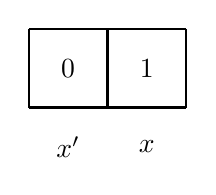
\begin{tikzpicture}
        \draw[thick] (0,0)--(2,0);
        \draw[thick] (0,0)--(0,1);
        \draw[thick] (0,1)--(2,1);
        \draw[thick] (2,0)--(2,1);
        \draw[thick] (1,0)--(1,1);
        \node at (0.5,0.5) {0};
        \node at (1.5,0.5) {1};
        \node at (0.5,-0.5) {$ x' $};
        \node at (1.5,-0.5) {$ x $};
    \end{tikzpicture}
\end{center}
The variable is represented by the right square and its complement $ x' $ by the left square.

\emph{Case of 2 Variables}: For $ n = 2 $, the Boolean function is of two variable, say $ x $ and $ y $. We have $ 2^2 = 4 $ squares, that is, a $ 2 \times 2 $ matrix of squares. Each squares contain one possible input from $ B_2 $.

The variable $ x  $ appears in the first row of the matrix as $ x' $ whereas $ x $ appears in the second row as $ x $. Similarly, $ y $ appears in the first column as $ y' $ and as y in the second column.
\begin{figure}[H]
    \centering
    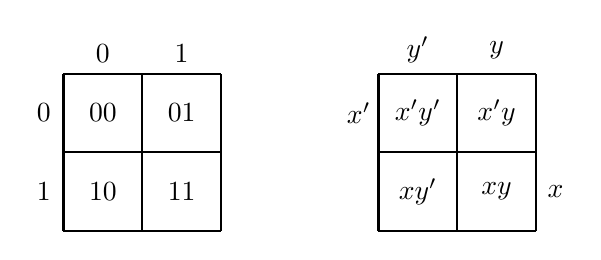
\begin{tikzpicture}
        \draw[thick] (0,0) grid (2,2);
        \node at (0.5,0.5) {10};
        \node at (1.5,0.5) {11};
        \node at (0.5,1.5) {00};
        \node at (1.5,1.5) {01};
        \node at (0.5,2.25) {0};
        \node at (1.5,2.25) {1};
        \node at (-0.25,1.5) {0};
        \node at (-0.25,0.5) {1};
        
        \draw[thick] (4,0) grid (6,2);
        \node at (4.5,0.5) {$xy'$};
        \node at (5.5,0.5) {$xy$};
        \node at (4.5,1.5) {$x'y'$};
        \node at (5.5,1.5) {$x'y$};
        \node at (4.5,2.3) {$y'$};
        \node at (5.5,2.3) {$y$};
        \node at (3.75,1.5) {$x'$};
        \node at (6.25,0.5) {$x$};
        \end{tikzpicture}
        \caption{2 variable Karnaugh Map}
\end{figure}
In this case, $ x $ is represented by the points in lower half of the map and $ y $ is represented by the points in the right half of the map.
\begin{defn}
    Two fundamental products are said to be \emph{adjacent} if they have the same variables and if they differ in exactly one literal. Thus, there must be an uncomplemented variable in one product which is complemented in the other.
\end{defn}
For example, if $ P_1 = x y z' $ and $ P_2 = x y' z'  $, then they are adjacent.\\
The sum of two such adjacent products will be a fundamental product with one less literal.\\
For example, in the case of above-mentioned adjacent products,
\[
    P_1+P_2=xyz'+xy'z'=xz'(y+y')=xz'(1)=xz'
\]
We note that two squares in Karnaugh map above are adjacent if and only if squares are geometrically adjacent, that is, have a side in common.

We know that a complete sum-of-products Boolean expression $ E(x, y) $ is a sum of minterms and hence can be represented in the Karnaugh map by placing checks in the appropriate square. A prime implicant of $ E(x, y) $ will be either a pair of adjacent squares in $ E $ or an isolated square (a square which is not adjacent to other square of $ E(x,y) $). A minimal sum of products for $ E(x,y) $ will consists of a minimum number of a prime implicants which cover all the square of $ E(x,y) $.
\begin{prob}
    Find the prime implicants and a minimal sum-of-products form from each of the following complete sum-of-products Boolean expression:
    \begin{enumerate}[label=(\alph*)]
        \item $ E_1=xy+xy' $
        \item $ E_2=xy+x'y+x'y' $
        \item $ E_3=xy+x'y' $
    \end{enumerate}
\end{prob}
\newpage
\begin{soln}
    \hfill
    \begin{enumerate}[label=(\alph*)]
        \item The Karnaugh map for $ E_1 $ is
        \begin{center}
            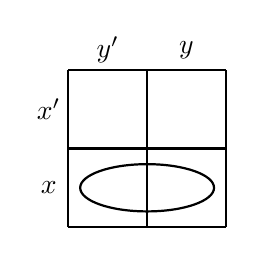
\begin{tikzpicture}
                \draw[thick] (0,0) grid (2,2);
                \node at (0.5,0.5) {\checkmark};
                \node at (1.5,0.5) {\checkmark};
                \node at (0.5,2.25) {$y'$};
                \node at (1.5,2.25) {$y$};
                \node at (-0.25,1.5) {$x'$};
                \node at (-0.25,0.5) {$x$};
                \draw[thick] (1,0.5)circle[x radius=.85, y radius=.3];
                \end{tikzpicture}
        \end{center}
        Check the squares corresponding to $ x y $ and $ x y' $. We note that $ E_1 $ consists of one prime implicant, the two adjacent square designated by the loop. The pair of adjacent square represents the variable $ x $. So $ x $ is the only prime implicant of $ E_1 $. Consequently, $ E_1 = x $ is its minimal sum.
        \item The Karnaugh map for $ E_2 $ is
        \begin{center}
            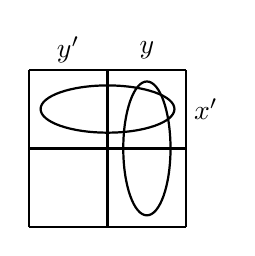
\begin{tikzpicture}
                \draw[thick] (0,0) grid (2,2);
                \node at (1.5,0.5) {\checkmark};
                \node at (0.5,1.5) {\checkmark};
                \node at (1.5,1.5) {\checkmark};
                \node at (0.5,2.25) {$y'$};
                \node at (1.5,2.25) {$y$};
                \node at (2.25,1.5) {$x'$};
                \draw[thick] (1,1.5)circle[x radius=.85, y radius=.3];
                \draw[thick] (1.5,1)circle[x radius=.3, y radius=.85];
                \end{tikzpicture}
        \end{center}
        Check the squares corresponding to $ x y $, $ x' y $, $ x' y' $. The expression $ E_2 $ contains two pairs of adjacent squares (designated by two loops) which include all the squares of $ E_2 $. The vertical pair represents $ y $ and the horizontal pair $ x' $. Hence, $ y $ and $ x $ are the prime implicants of $ E_2 $. Thus, $ E_2(x,y)=x'+y $ is minimal sum.
        \item The Karnaugh map for $ E_3 $ is
        \begin{center}
            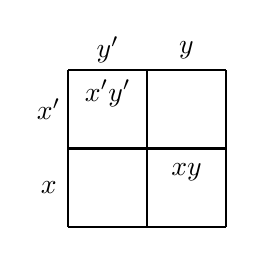
\begin{tikzpicture}
                \draw[thick] (0,0) grid (2,2);
                \node at (1.5,0.7) {$xy$};
                \node at (1.5,0.3) {\checkmark};
                \node at (0.5,1.3) {\checkmark};
                \node at (0.5,1.7) {$x'y'$};
                \node at (0.5,2.25) {$y'$};
                \node at (1.5,2.25) {$y$};
                \node at (-0.25,1.5) {$x'$};
                \node at (-0.25,0.5) {$x$};
                \end{tikzpicture}
        \end{center}
        Check (tick) the squares corresponding to $ x y $ and $ x' y' $. The expression $ E_3 $ consists of two isolated squares which represent $ x y $ and $ x' y' $. Hence $ x y $ and $ x ' y' $ are the prime implicants of $ E_3 $ and so $ E_3 = x y + x' y' $ is its minimal sum.
    \end{enumerate}
\end{soln}


\emph{Case of 3 variables}: We now turn to the case of a function $ f: B_3 \to B $ which is function of $ x $, $ y $ and $ z $. The Karnaugh map corresponding to Boolean expression $ E(x, y, z) $ is shown in the diagram below:
\begin{center}
    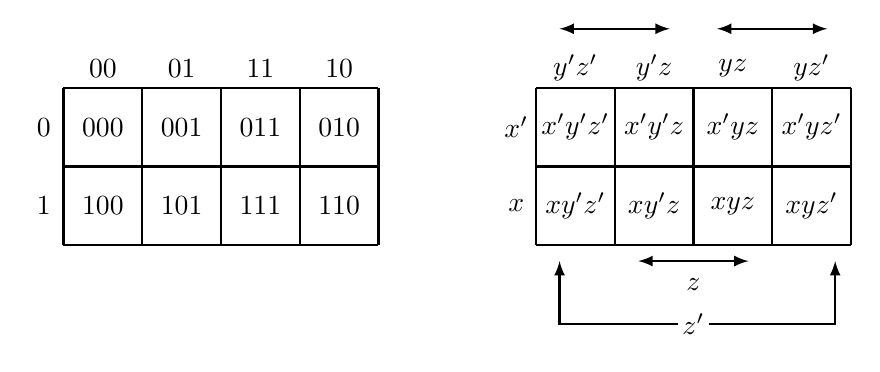
\begin{tikzpicture}
        \draw[thick] (0,0) grid (4,2);
        \node at (0.5,0.5) {100};
        \node at (1.5,0.5) {101};
        \node at (2.5,0.5) {111};
        \node at (0.5,1.5) {000};
        \node at (1.5,1.5) {001};
        \node at (2.5,1.5) {011};
        \node at (3.5,1.5) {010};
        \node at (3.5,0.5) {110};
        \node at (0.5,2.25) {00};
        \node at (1.5,2.25) {01};
        \node at (2.5,2.25) {11};
        \node at (3.5,2.25) {10};
        \node at (-0.25,1.5) {0};
        \node at (-0.25,0.5) {1};
        
        
        \draw[thick] (6,0) grid (10,2);
        \node at (6.5,0.5) {$xy'z'$};
        \node at (7.5,0.5) {$xy'z$};
        \node at (8.5,0.5) {$xyz$};
        \node at (6.5,1.5) {$x'y'z'$};
        \node at (7.5,1.5) {$x'y'z$};
        \node at (8.5,1.5) {$x'yz$};
        \node at (9.5,1.5) {$x'yz'$};
        \node at (9.5,0.5) {$xyz'$};
        \node at (6.5,2.25) {$y'z'$};
        \node at (7.5,2.25) {$y'z$};
        \node at (8.5,2.25) {$yz$};
        \node at (9.5,2.25) {$yz'$};
        \node at (5.75,1.5) {$x'$};
        \node at (5.75,0.5) {$x$};
        \node at (8,-0.5) {$z$};
        \node at (8,-1.0) {$z'$};
        \draw[thick,latex-latex] (6.3,2.75)--(7.7,2.75);
        \draw[thick,latex-latex] (8.3,2.75)--(9.7,2.75);
        \draw[thick,latex-latex] (7.3,-0.2)--(8.7,-0.2);
        \draw[thick,latex-] (6.3,-0.2)|-(7.8,-1.0);
        \draw[thick,-latex] (8.2,-1.0)-|(9.8,-0.2);
        \end{tikzpicture}
\end{center}
Here $ x $, $ y $, $ z $ are respectively represented by lower half, right half and middle two quarters of the map.\\
Similarly, $ x' $, $ y'  $,$  z' $ are respectively represented by upper half, left half and left and right quarter of the map.
\begin{defn}
    By a Basic Rectangle in the Karnaugh map with three variables, we mean a square, two adjacent squares or four squares which form a one-by four, or a two by-two rectangle. These basic rectangles correspond to fundamental products of three, two and one literal respectively.
\end{defn}

Further, the fundamental product represented by a basic rectangle is the product of just those literals that appear in every square of the rectangle.

Let a complete sum of products Boolean expression $ E(x, y, z) $ is represented in the Karnaugh map by placing checks in the appropriate squares. A prime implicant of $ E $ will be a maximal basic rectangle of $ E $, i.e., a basic rectangle contained in $ E $ which is not contained in any larger basic rectangle in $ E $.

A minimal sum-of-products form for $ E $ will consist of a minimal cover of $ E $, i.e., a minimal number of maximal basic rectangles of $ E $ which together include all the square of $ E $.
\begin{prob}
    Find the prime implicants and a minimal sum-of-products form for each of the following complete sum-of-products Boolean expressions:
    \begin{enumerate}[label=(\alph*)]
        \item $ E_1 = xyz + xyz' + x' yz' + x' y' z $.
        \item $ E_2 = xyz + xyz' + xy' z + x' yz + x' y' z $.
        \item $ E_3 = xyz + xyz' + x' yz + x' y' z $.
    \end{enumerate}
\end{prob}
\begin{soln}
    \hfill
    \begin{enumerate}[label=(\alph*)]
        \item The Karnaugh map for $ E_1 $ is
        \begin{center}
            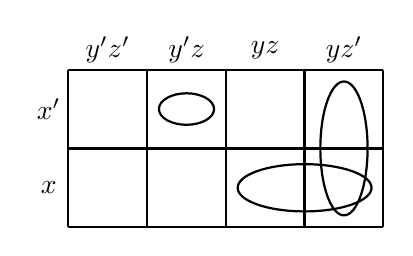
\begin{tikzpicture}
                \draw[thick] (0,0) grid (4,2);
                \node at (2.5,0.5) {\checkmark};
                \node at (3.5,0.5) {\checkmark};
                \node at (1.5,1.5) {\checkmark};
                \node at (3.5,1.5) {\checkmark};
                        
                \node at (0.5,2.25) {$y'z'$};
                \node at (1.5,2.25) {$y'z$};
                \node at (2.5,2.25) {$yz$};
                \node at (3.5,2.25) {$yz'$};
                \node at (-0.25,1.5) {$x'$};
                \node at (-0.25,0.5) {$x$};
                \draw[thick] (1.5,1.5)circle[x radius=.35, y radius=.2];
                \draw[thick] (3,0.5)circle[x radius=.85, y radius=.3];
                \draw[thick] (3.5,1)circle[x radius=.3, y radius=.85];
                \end{tikzpicture}
        \end{center}
        We check the four squares corresponding to four summands in $ E_1 $. Here $ E_1 $ has three prime implicants (maximal basic rectangles) which are encircled. These are $ x y $, $ y z' $ and $ x' y' z $. All three are needed to cover $ E_1 $. Hence, minimal sum for $ E_1 $ is $ E_1=xy+yz'+x'y'z $.
        \item The Karnaugh map for $ E_2 $ is
        \begin{center}
            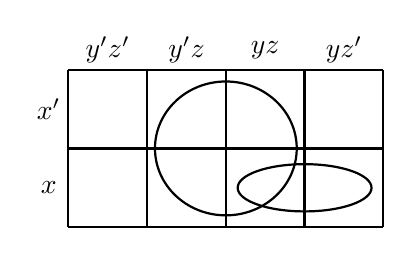
\begin{tikzpicture}
                \draw[thick] (0,0) grid (4,2);
                % \node at (0.5,0.5) {100};
                \node at (1.5,0.5) {\checkmark};
                \node at (2.5,0.5) {\checkmark};
                \node at (3.5,0.5) {\checkmark};
                % \node at (0.5,1.5) {000};
                \node at (1.5,1.5) {\checkmark};
                \node at (2.5,1.5) {\checkmark};
                % \node at (3.5,1.5) {\checkmark};
                        
                \node at (0.5,2.25) {$y'z'$};
                \node at (1.5,2.25) {$y'z$};
                \node at (2.5,2.25) {$yz$};
                \node at (3.5,2.25) {$yz'$};
                \node at (-0.25,1.5) {$x'$};
                \node at (-0.25,0.5) {$x$};
                \draw[thick] (3,0.5)circle[x radius=.85, y radius=.3];
                \draw[thick] (2,1)circle[x radius=.9, y radius=.85];
                \end{tikzpicture}
        \end{center}
        Check the squares corresponding to the five summands. $ E_2 $ has two prime implicants which are circled. One is the two adjacent squares which represent $ x y $, and the other is the two-by-two square which represents $ z $. Both are needed to cover $ E_2 $ so the minimal sum for $ E_2 $ is $ E_2=xy+z $.\newpage
        \item The Karnaugh map for $ E_3 $ is
        \begin{center}
            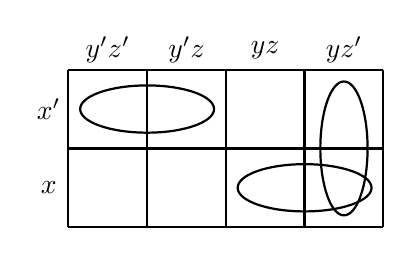
\begin{tikzpicture}
                \draw[thick] (0,0) grid (4,2);
                % \node at (0.5,0.5) {100};
                % \node at (1.5,0.5) {\checkmark};
                \node at (2.5,0.5) {\checkmark};
                \node at (3.5,0.5) {\checkmark};
                
                \node at (0.5,1.5) {\checkmark};
                \node at (1.5,1.5) {\checkmark};
                % \node at (2.5,1.5) {\checkmark};
                \node at (3.5,1.5) {\checkmark};
                        
                \node at (0.5,2.25) {$y'z'$};
                \node at (1.5,2.25) {$y'z$};
                \node at (2.5,2.25) {$yz$};
                \node at (3.5,2.25) {$yz'$};
                \node at (-0.25,1.5) {$x'$};
                \node at (-0.25,0.5) {$x$};
                \draw[thick] (3,0.5)circle[x radius=.85, y radius=.3];
                \draw[thick] (1,1.5)circle[x radius=.85, y radius=.3];
                \draw[thick] (3.5,1)circle[x radius=.3, y radius=.85];
                \end{tikzpicture}
        \end{center}
        Check the squares corresponding to the five summands. Here $ E_3 $ has three prime implicants $ x y $, $ yz' $, $ x' y' $. All these are needed in a minimal cover of $ E_3 $. Hence, $ E_3 $ has minimal sum as $ E_3=xy+yz'+x'y' $.
    \end{enumerate}
\end{soln}
\begin{rem}
    To find the fundamental product represented by a basic rectangle, find literals which appear in all the squares of the rectangle.
\end{rem}


\emph{Case of 4 variables}: We consider a Boolean function $ f : B_4 \to B $, considered as a function of $ x $, $ y $, $ z $ and $ t $. Each of the 16 squares $ (2^4) $ corresponds to one of the minterms with four variables.
\[
    xyzt,\;xyzt', \dot, x'yz't
\]

We consider first and last columns to be adjacent, and first and last rows to be adjacent, both by Wrap around, and we look for rectangles with sides of length some power of 2, so the length is 1, 2 or 4. The expression for such rectangles is given by intersecting the large labelled rectangles.
\begin{center}
    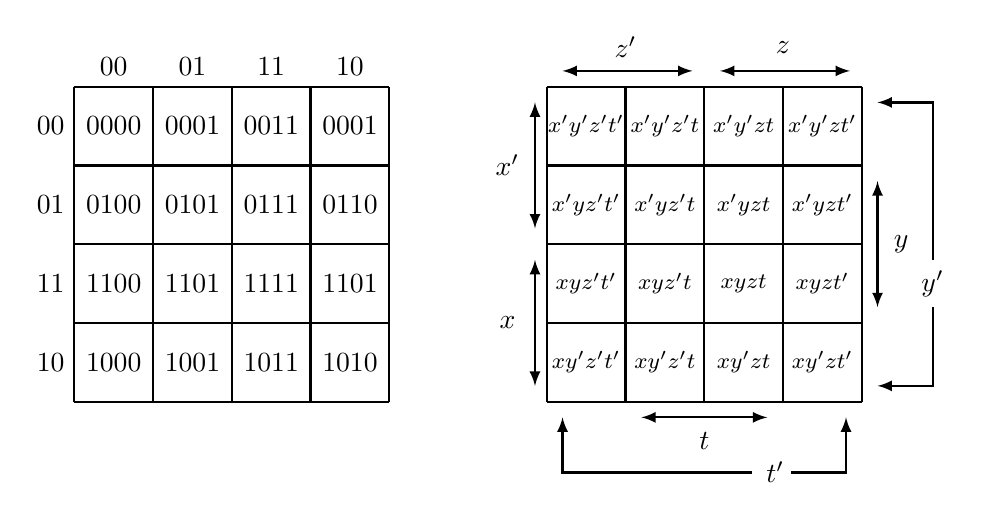
\begin{tikzpicture}
        \draw[thick] (0,0) grid (4,4);
        \node at (0.5,0.5) {1000};
        \node at (1.5,0.5) {1001};
        \node at (2.5,0.5) {1011};
        \node at (3.5,0.5) {1010};
        
        \node at (0.5,1.5) {1100};
        \node at (1.5,1.5) {1101};
        \node at (2.5,1.5) {1111};
        \node at (3.5,1.5) {1101};
                
        \node at (0.5,2.5) {0100};
        \node at (1.5,2.5) {0101};
        \node at (2.5,2.5) {0111};
        \node at (3.5,2.5) {0110};
        
        \node at (0.5,3.5) {0000};
        \node at (1.5,3.5) {0001};
        \node at (2.5,3.5) {0011};
        \node at (3.5,3.5) {0001};
        
        \node at (0.5,4.25) {00};
        \node at (1.5,4.25) {01};
        \node at (2.5,4.25) {11};
        \node at (3.5,4.25) {10};
        
        \node at (-0.3,3.5) {00};
        \node at (-0.3,2.5) {01};
        \node at (-0.3,1.5) {11};
        \node at (-0.3,0.5) {10};
        
        \draw[thick] (6,0) grid (10,4);
        \node at (6.5,0.5) {\footnotesize$xy'z't'$};
        \node at (7.5,0.5) {\footnotesize$xy'z't$};
        \node at (8.5,0.5) {\footnotesize$xy'zt$};
        \node at (9.5,0.5) {\footnotesize$xy'zt'$};
        
        \node at (6.5,1.5) {\footnotesize$xyz't'$};
        \node at (7.5,1.5) {\footnotesize$xyz't$};
        \node at (8.5,1.5) {\footnotesize$xyzt$};
        \node at (9.5,1.5) {\footnotesize$xyzt'$};
        
        \node at (6.5,2.5) {\footnotesize$x'yz't'$};
        \node at (7.5,2.5) {\footnotesize$x'yz't$};
        \node at (8.5,2.5) {\footnotesize$x'yzt$};
        \node at (9.5,2.5) {\footnotesize$x'yzt'$};
        
        \node at (6.5,3.5) {{\footnotesize $x'y'z't'$}};
        \node at (7.5,3.5) {\footnotesize$x'y'z't$};
        \node at (8.5,3.5) {\footnotesize$x'y'zt$};
        \node at (9.5,3.5) {\footnotesize$x'y'zt'$};
        
        \node at (5.5,01) {$x$};
        \draw[thick,latex-latex] (5.85,.2)--(5.85,1.8);
        \node at (5.5,3) {$x'$};
        \draw[thick,latex-latex] (5.85,2.2)--(5.85,3.8);
        \node at (7,4.5) {$z'$};
        \draw[thick,latex-latex] (6.2,4.2)--(7.85,4.2);
        \node at (9,4.5) {$z$};
        \draw[thick,latex-latex] (8.2,4.2)--(9.85,4.2);
        \draw[thick,latex-latex] (10.2,1.2)--(10.2,2.8);
        \node at (10.5,2) {$y$};
        \node at (10.9,1.5) {$y'$};
        \draw[thick,-latex] (10.9,1.2)|-(10.2,0.2);
        \draw[thick,-latex] (10.9,1.8)|-(10.2,3.8);
        \node at (8,-0.5) {$t$};
        \draw[thick,latex-latex] (7.2,-0.2)--(8.8,-0.2);
        \node at (8.9,-0.9) {$t'$};
        \draw[thick,-latex] (9.1,-0.9)-|(9.8,-0.2);
        \draw[thick,-latex] (8.6,-0.9)-|(6.2,-0.2);
        \end{tikzpicture}
\end{center}
A basic rectangle in a four variable Karnaugh map is a square, two adjacent squares, four squares which form one-by-four or two by two rectangle or eight square squares which form a two by four rectangles. These rectangles correspond to fundamental product with four, three, two and one literal respectively. Maximal basic rectangles are prime implicants.
\begin{prob}
    Find the fundamental product $ P $ represented by the basic rectangle in the Karnaugh map given below:
    \begin{center}
        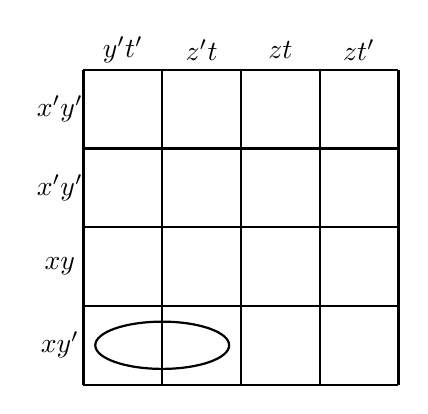
\begin{tikzpicture}
            \draw[thick] (0,0) grid (4,4);
            \node at (0.5,0.5) {\checkmark};
            \node at (1.5,0.5) {\checkmark};
                    
            \node at (0.5,4.25) {$y't'$};
            \node at (1.5,4.25) {$z't$};
            \node at (2.5,4.25) {$zt$};
            \node at (3.5,4.25) {$zt'$};
            \node at (-0.3,3.5) {$x'y'$};
            \node at (-0.3,2.5) {$x'y'$};
            \node at (-0.3,1.5) {$xy$};
            \node at (-0.3,0.5) {$xy'$};
            \draw[thick] (1,0.5)circle[x radius=.85, y radius=.3];
            \end{tikzpicture}
    \end{center} 
\end{prob}
\begin{soln}
    We find the literals which appear in all the squares of the basic rectangle. Then $ P $ will be the product of such literals.\\
    Here $ x $, $ y'  $, $ z $ appear in both squares. Hence,
    \[P = x y' z'\]
    is the fundamental product represented by the basic rectangle in question.
\end{soln}
\end{document}